\documentclass{article}
\usepackage[utf8]{inputenc}
\usepackage{amsmath}
\usepackage{amsthm}
\usepackage{graphicx}
\usepackage{geometry}
\usepackage{caption}
\usepackage{hyperref}
\usepackage{minted}
\usemintedstyle{manni}
\geometry{a4paper, portrait, margin=1in}

\theoremstyle{plain}
\newtheorem{thm}{Theorem}

\theoremstyle{definition}
\newtheorem{defn}{Definition} % definition numbers are dependent on theorem numbers
\newtheorem{exmp}{Example} % same for example numbers

\hypersetup{
    colorlinks=true,
    urlcolor=blue,
}

\title{Operating Systems (UE18CS302)\\
    \large Unit 4}
\author{Aronya Baksy}
\date{October 2020}

\begin{document}
    \maketitle
\section{Mass-Storage Structures}
\subsection{Magnetic Disk Drive}
\begin{itemize}
    \item These consist of \textbf{platters} (with diameter between 1.8in and 3.5in) stacked one on top of another, about a common central axis. The drive motor spins the central axis at a rate specified in RPM (Rotations per minute). 
    
    \item Each platter is coated with a magnetic material, and all information is stored on this magnetic coating (using the principle of hysteresis). 
    
    \item There is a \textbf{read -write head} for each platter. All the read-write heads are moved all together by the \textbf{disk arm}.  
    
    \item Each platter is divided into concentric circular regions called \textbf{tracks}. The set of all the tracks in the disk, at one position of the arm, is called a \textbf{cylinder}. 
    
    \item Each circular track on each platter, is divided into \textbf{sectors}. 
\end{itemize}
\begin{figure}[!h]
    \centering
    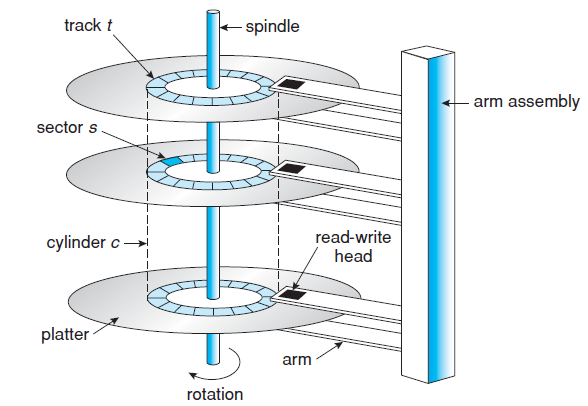
\includegraphics[scale=0.5]{os1.png}
    \caption{Structure of a Magnetic Disk Drive}
    \label{0}
\end{figure}
\begin{itemize}
    \item The \textbf{access time} is composed of the following parts:
    \begin{enumerate}
    
        \item The \textbf{transfer time} is the time needed to transfer one unit of data from the disk to the memory. $t_{transfer}$
        
        \item Time needed to move the arm to the correct cylinder, called the \textbf{seek time} $t_{seek}$
        
        \item Time needed for the desired sector to move to the read-write head, called the \textbf{rotational latency}. $t_{\text{avg rot latency}}$
        
        \item Latency of the controller operation (the mechanical controller that controls the arm assembly), called the \textbf{controller time} $t_{controller}$
        
    \end{enumerate}
    
    \item The seek time and controller time are generally predefined constant values. The transfer time and rotational latency depends on the disk characteristics such as its rotation speed and the layout of tracks/sectors on the platters. 
    
    \item Formulae:
    \begin{align*}
        \text{Data Transfer Rate} &= RPS \times \text{track capacity} \times \text{num of surfaces}\\
        t_{transfer} &= \text{Amount of data to be transferred}\times \text{Data Transfer Rate}\\
        t_{\text{avg rot latency}} &= \frac{\text{Time period of rotation}}{2}\\
        \text{Disk Access time} &= t_{seek} + t_{\text{avg rot latency}} + t_{transfer} + t_{controller}
    \end{align*}
    
    \item The situation where the read-write head makes actual contact with the platter, thus damaging the platter, is called \textbf{head crash}. This generally results in the entire disk being replaced. 
    
    \item Most common rotation speeds for disk drives are 5400 RPM and 7200 RPM. A 7200RPM drive would deliver data at a 33\% faster rate compared to a 5400 RPM drive given the same areal density of bits. 
    
    \item Disk drive is connected to the computer by an \textbf{I/O Bus}. Bus technologies include \textbf{ATA}, Serial ATA (\textbf{SATA}), \textbf{USB} and \textbf{Fibre Channel}. 
    
    \item Disk operation is coordinated by a \textbf{host controller} in the computer and a \textbf{disk controller} in the disk drive.
    
    \item When the CPU requests for some memory location, it places the appropriate command in the host controller. From the host controller this command is transferred to the disk controller via the I/O Bus. The disk controller operates the disk hardware to service the request.
    
    \item Disk controllers have an inbuilt cache, hence transfers within the disk take place between the disk surface and the cache, while transfers from disk to computer take place between the cache and the host controller at electronic speeds. 
\end{itemize}

\subsection{Solid State Drive}
\begin{itemize}
    \item Non-volatile memory that is used for permanent storage. Variations of this technology include flash storage, and DRAM with an external power supply to help it maintain its state. 
    
    \item \textbf{Advantages}: No moving parts in an SSD, hence more reliable and faster due to no seek time and rotational latency. They are also more power efficient.
    
    \item \textbf{Disadvantages}: Higher cost per MB than traditional disk drives, they have less capacity than a disk drive of the similar size, and they have a shorter lifespan. 
    
    \item Due to the large speed of SSDs, the I/O bus speed is a performance bottleneck. Hence some SSDs are designed to connect directly to the system bus (using technologies like PCI). 
    
    \item SSDs are being used either as replacements for disk drives, or as an additional cache tier ahead of a disk drive. 
\end{itemize}

\subsection{Magnetic Tape}
\begin{itemize}
    \item This is a relatively permanent storage medium (compared to SSDs) but suffers from slow random access time compared to both SSDs and magnetic disk drives. 
    
    \item Tapes are used mainly for backup, for storage of infrequently used information, and as a medium for transferring information from one system to another.
    
    \item A tape is kept in a spool and is wound or rewound past a read–write head. Moving to the correct spot on a tape can take minutes, but once positioned, tape drives can write data at speeds comparable to disk drives.
    
    \item Tape drive capacities can vary, with current versions having capacities in Terabyte range and some tapes have inbuilt compression for increasing the capacity.
\end{itemize}

\section{Disk Scheduling Algorithms}
\begin{itemize}
    \item These algorithms aim to minimize the seek time between requests for data in a particular cylinder.
\end{itemize}

\subsection{FCFS (First Come First Serve)}
\begin{itemize}
    \item The sequence of requests is treated as a queue, and the first one in the queue will be serviced first. This can also be called a FIFO algorithm. 
    
    \item The disadvantage is that if two consecutive requests are in far apart cylinders of the disk, then this leads to longer seek times.
\end{itemize}

\subsection{SSTF (Shortest Seek Time First)}
\begin{itemize}
    \item The request that is closest to the current position of the read-write head will be served next in this algorithm.
    
    \item The disadvantage is that of starvation, where requests that are far away from the current head position may be delayed because of new requests coming in that are closer to the current head position.
\end{itemize}

\subsection{SCAN and C-SCAN(Elevator Algorithm)}
\begin{itemize}
    \item The read-write head starts from one end of the disk, servicing the requests as it moves on to one side of the disk. 
    
    \item As it reaches the end, the head reverses and services the requests on this path. 
    
    \item C-SCAN, or Circular SCAN is similar to SCAN, but once the head reaches one end, it tracks back to the other end instead of servicing disk requests while going back. 
\end{itemize}

\subsection{LOOK and C-LOOK}
\begin{itemize}
    \item Instead of travelling all the way to the ends of the disk, the disk head only travels till the farthest request and then goes back to the other end, instead of going all the way to the last cylinder of the disk.
    
    \item In Circular LOOK (C-LOOK), the disk head skips to the other end without servicing any requests on the return trip. 
\end{itemize}

\section{Swap-Space Management}
\begin{itemize}
    \item Pages are swapped out of main memory when the usage of main memory reaches a critically high level. 
    
    \item The use of swap space means that the disk (ie. the swap space part of the disk) is treated as an extension of the main memory. As disk access is slower than main memory access, hence swapping leads to a decrease in performance. 
\end{itemize}

\subsection{Size of Swap Space}
\begin{itemize}
    \item In systems that swap out entire processes instead of pages, the swap space has to be large enough to hold entire process images (code, global variables, stack, heap etc.). On the other hand, systems that only swap pages would need less amount of swap space.  
    
    \item Overestimating swap space is safer than underestimating it, as that can lead to processes crashing because of swap space running out. 
    
    \item On Solaris, swap space is set to the amount by which virtual memory exceeds the pageable physical memory. On Linux, the earlier recommendation was to set swap space as double the size of physical memory, but modern Linux versions use less swap space. 
    
    \item Some OSes allow multiple swap spaces (including files and dedicated swap partitions) across multiple disks so that the I/O can be spread evenly across the entire bandwidth of the system. 
\end{itemize}

\subsection{Location of Swap Space}
\begin{itemize}
    \item One implementation is to have the swap space as \textbf{part of the file system itself}, as one large contiguous file. This allows the use of normal file-system routines to create, allocate and rename it.
    
    \item This approach is inefficient, as it leads to more disk accesses during traversal of the file-system and allocation data structures. 
    
    \item External fragmentation can also increase swap time due to multiple seeks needed while accessing an entire process image. 
    
    \item The alternative to this implementation is to have a \textbf{separate raw partition} for the swap space. 
    
    \item No file system or directory structure exists in this space, a separate swap-space manager is used to allocate and deallocate blocks from it. Here speed is more important than storage efficiency, as swap space is used very frequently compared to disk. 
    
    \item This approach can cause internal fragmentation, but it is short lived because the swap space is reinitialized at boot time. 
    
    \item This approach fixes the swap space, and changing its size would mean allocating the file system partitions elsewhere, or deleting them totally, or adding swap space in another disk. 
    
    \item Modern OSes like new versions of Linux allow the admin to decide whether to swap to the file system (easy to implement and convenient) or to a raw partition (hard to implement but increased speed)
\end{itemize}

\subsection{Examples of Swap Space Management}
\begin{itemize}
    \item In old versions of UNIX (that do not use paging), entire processes would be copied between contiguous disk regions, and the main memory. Later versions of UNIX used paging and swapping to handle page faults, as more hardware was introduced.
    
    \item In Solaris 1, swap space is used only for pages of \textbf{anonymous memory}, ie. memory that is not backed to any file name in the file system. This includes stack/heap/uninitialized data of a process. 
    
    \item For text files containing process code, the files are read directly from the file system on disk to the main memory, and thrown out if not needed. These pages are directly accessed from disk as it is more efficient to re-read directly from disk than to first write to swap space and then re-read it from there. 
    
    \item In later versions of Solaris, swap space is only created when a page is removed from main memory, rather than when the virtual memory page is first created. This is more efficient on modern computers that have large amounts of physical memory, and hence undergo less paging.
    
    \item \textbf{Linux} also uses swap space only for anonymous memory, allows for multiple swap spaces and allows them to reside in either the file system or a separate partition. 
    
    \item The swap space in Linux is divided into page slots (each of size 4KB, same as page size), that hold the swapped pages.
    
    \item The \textbf{swap map} is an array of counters (one element per page slot) that determines the number of processes that map to the swapped page. A value of 0 indicates that the slot is free, value more than 1 indicates a shared page between multiple processes. 
\end{itemize}

\section{RAID (Redundant Array of Independent Disks)}
\begin{itemize}
    \item RAID is a storage virtualization technology that presents an array of multiple independent disks as a single contiguous storage to the CPU.
    
    \item Its primary advantage is allowing disk accesses in parallel and increasing redundancy of the disk storage (to reduce the impact of a failure). 
\end{itemize}

\subsection{Redundancy in RAID}
\begin{itemize}
    \item One basic technique to include redundancy in the design of RAID is \textbf{mirroring}, where one logical disk consists of 2 actual physical disks. A write to this disk would mean writing the same data to both disks.
    
    \item In a \textbf{mirrored volume}, if one disk fails, the other one is used in its place. Data is lost only if the second disk fails before the first one can be replaced.
    
    \item eg: Let mean time of failure for a single disk be 100,000 hours. For an array of 100 disks, the mean time of failure would be 100000/100  = 1000 hours = 41.66 days.
    
    \item For a mirrored system of 2 independent disks each having mean time to failure of 100,000 hours and mean time of replacement as 10 hours, the mean time of failure for this system is $\frac{100,000^2}{2 \times 10}  \approx 57,000$ years.
    
    \item In real life the independence assumption is not valid as disks that are close to each other are prone to failure (eg: due to natural disasters, power failures, manufacturing defects within a batch, age related issues). 
    
    \item In case a power failure occurs in the middle of a write operation, the data in each disk may be in an inconsistent state. 
    
    \item One solution to this is to perform writes in sequence (write to one disk fully then the next one).
    
    \item Another solution is to write to a non-volatile solid state cache memory (NVRAM) that is protected from data loss during power failures, hence writes can be considered complete at that point (assuming that NVRAM has error correction and protection).
\end{itemize}

\subsection{Parallelism in RAID}
\begin{itemize}
    \item In mirroring, the number of reads serviced per unit time is double as there are $N$ disks that can service a given request. The actual transfer time is same as a single disk setup. 
    
    \item The transfer rate can be improved using \textbf{striping}. 
    
    \item In \textbf{bit-level striping}, the bits of each byte are split across the disks. (eg: if there are 8 disks then the $i$th bit of every byte is assigned to the $i$th disk)
    
    \item In \textbf{block-level striping} considering $N$ disks in RAID, block $i$ of a file goes to disk $i\text{ mod }N$. 
    
    \item All the disks in the array participate in the disk access, so number of accesses handled is the same as single disk setup, but access time is reduced $\frac{1}{N}$ times as $N$ disks are simultaneously supplying data.  
    
    \item Disk parallelism has 2 main goals: \textbf{increase throughput} of small accesses, \textbf{reduce access time} for large accesses. 
\end{itemize}

\subsection{Levels of RAID}
\begin{itemize}
    \item These are techniques that combine mirroring (increase reliability but increase cost as well) and striping (increase parallelism but no improvement in reliability), along with other techniques like error correction and parity bits. 
    
    \item Each level of RAID has a different trade-off between cost, performance and reliability.
\end{itemize}

\subsubsection{RAID 0}
\begin{itemize}
    \item Disk array with block-level striping only.
\end{itemize}

\begin{figure}[!h]
    \centering
    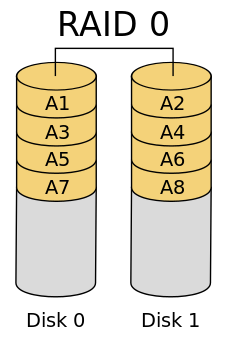
\includegraphics[scale=0.3]{raid0.png}
    \caption{RAID 0}
    \label{fig:my_label}
\end{figure}

\subsubsection{RAID 1}
\begin{itemize}
    \item Disk array with disk mirroring only
\end{itemize}

\begin{figure}[!h]
    \centering
    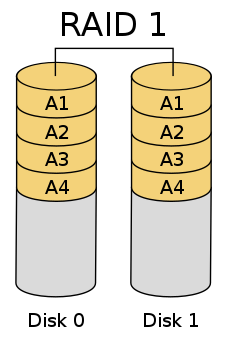
\includegraphics[scale=0.3]{raid1.png}
    \caption{RAID 1}
    \label{fig:my_label_1}
\end{figure}

\subsubsection{RAID 2}
\begin{itemize}
    \item Disk array with \textbf{memory-style error correction code} (ECC) and bit level striping. 
    
    \item For an error correction code like the $Hamming(7,4)$ code that attaches 3 parity bits to the 4 data bits, there would be a 3-disk overhead on top of the 4 disks needed to store the 4 data bits.
    
    \item In case of a single disk failure, the rest of the bits in that byte can be read from the other disks, and the missing bit can be reconstructed ($Hamming(7,4)$ can correct single bit errors or detect 2/3 bit errors). 
    
\end{itemize}

\begin{figure}[!h]
    \centering
    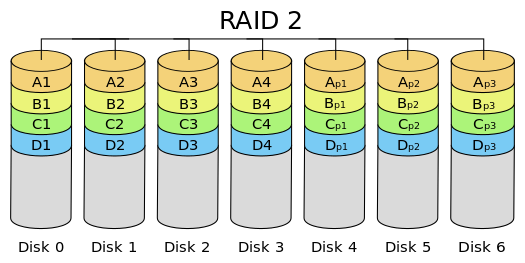
\includegraphics[scale=0.4]{raid2.png}
    \caption{RAID 2}
    \label{fig:my_label_2}
\end{figure}

\subsubsection{RAID 3}
\begin{itemize}
    \item This level uses \textbf{Bit-interleaved parity organization}, wherein the parity information is stored on a single disk instead of being interleaved with the data. 
    
    \item A single parity bit can be used for both error correction and detection because disk controllers can detect whether a read/write happened correctly or not (unlike memory controllers). 
    
    \item RAID 3 offers lower read time than RAID 1 (because of striping which is not present in RAID 1) and uses less number of disks, but can service less I/O operations per second as all the disks in RAID 3 need to take part in every I/O operation.
    
    \item The overheads of computing the parity bits (reducing disk performance) are handled by a dedicated RAID controller that offloads this job from the CPU. An NVRAM cache is also used in conjunction with this to buffer the reads/writes from the controller while the actual data is written to the disk. 
\end{itemize}

\begin{figure}[!h]
    \centering
    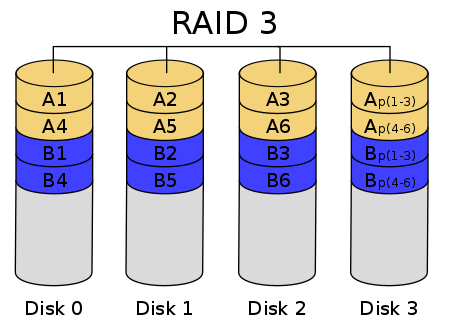
\includegraphics[scale=0.4]{raid3.png}
    \caption{RAID 3}
    \label{fig:my_label_3}
\end{figure}

\subsubsection{RAID 4}
\begin{itemize}
    \item This level uses \textbf{Block-interleaved parity organization}, wherein the parity block is stored on a separate disk and failed blocks can be restored from the correct ones. 
    
    \item A single block read accesses only one disk, hence rate of data transfer is less, but more I/O requests can be serviced in parallel.
    
    \item Small writes (data to be written is less than block size) are inefficient in RAID 4 as the entire block has to be copied to memory, modified and written back to the disk, while also modifying the corresponding parity block. 
    
    \item Large writes and reads are more efficient with RAID 4 than other levels of RAID due to the block-level parallelism.
\end{itemize}

\begin{figure}[!h]
    \centering
    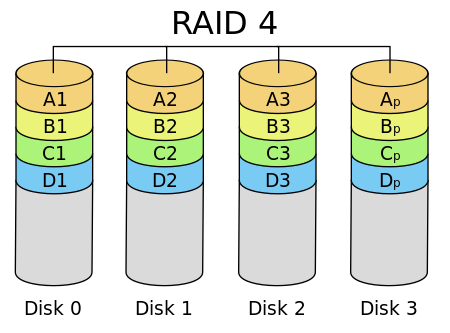
\includegraphics[scale=0.4]{raid4.png}
    \caption{RAID 4}
    \label{fig:my_label_4}
\end{figure}

\subsubsection{RAID 5}
\begin{itemize}
    \item This level uses \textbf{block-level distributed parity}. There is no dedicated parity disk, rather the parity for a particular set of blocks are randomly distributed across the disks.
    
    \item A parity block cannot store parity information for a block in the same disk, as failure of that disk leads to loss of data as well as parity making reconstruction of data impossible.
    
    \item RAID 5 distributes the stress of the parity disk (and its resulting overuse, which may occur in RAID 4) among all the $N+1$ disks in the RAID setup. 
\end{itemize}

\begin{figure}[!h]
    \centering
    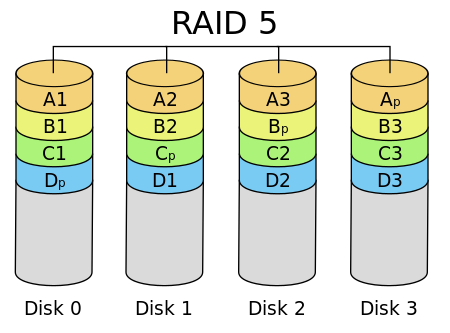
\includegraphics[scale=0.4]{raid5.png}
    \caption{RAID 5}
    \label{fig:my_label_5}
\end{figure}

\subsubsection{RAID 6}
\begin{itemize}
    \item Using 2 parity blocks instead of 1 as seen in RAID 5, RAID 6 can reconstruct data from at most 2 disk failures. Instead of parity-based ECC, codes like the \textbf{Reed-Solomon code} are used.  
    
    \item This is in contrast with RAID levels 2,3,4 and 5 that can only handle one drive failure max. 
    
    \item The disadvantage of RAID 6 is increased overhead in terms of number of disks needed. RAID 6 needs minimum of 4 disks to be used (in constrast to RAID 2,3,4 and 5 that need minimum 3 disks). 
\end{itemize}

\begin{figure}[!h]
    \centering
    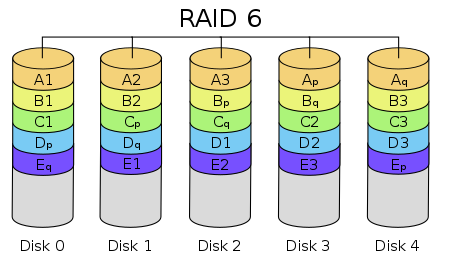
\includegraphics[scale=0.45]{raid6.png}
    \caption{RAID 6}
    \label{fig:my_label_6}
\end{figure}

\subsubsection{RAID 0+1 (or RAID 01)}
\begin{itemize}
    \item This level of RAID combines RAID 0 (striping) and RAID 1 (mirroring) in a way that it becomes a \textbf{mirror of stripes}.
    
    \item First the disks are striped, then they are mirrored. 
    
    \item RAID 0+1 has the advantage of performance (due to increased parallelism provided by RAID 0) as well as increased reliability (due to mirroring from RAID 1).
    
    \item The disadvantage of RAID 1 (ie. more disks needed) is also carried over, hence RAID 0+1 is expensive
\end{itemize}

\begin{figure}[!h]
    \centering
    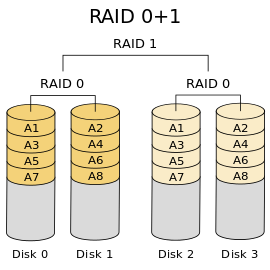
\includegraphics[scale=0.6]{raid01.png}
    \caption{RAID 0+1}
    \label{fig:my_label_7}
\end{figure}

\subsubsection{RAID 1+0 (or RAID 10)}
\begin{itemize}
    \item The operations are applied in the exact reverse order as RAID 01. First the disks are mirrored, then they are striped. 
    
    \item A single disk failure in RAID 0+1 renders that entire stripe inaccessible (it has to be read from its mirrored copy in the other disk). However, a single disk failure in RAID 1+0 means that the stripe is still accessible. 
\end{itemize}

\begin{figure}[!h]
    \centering
    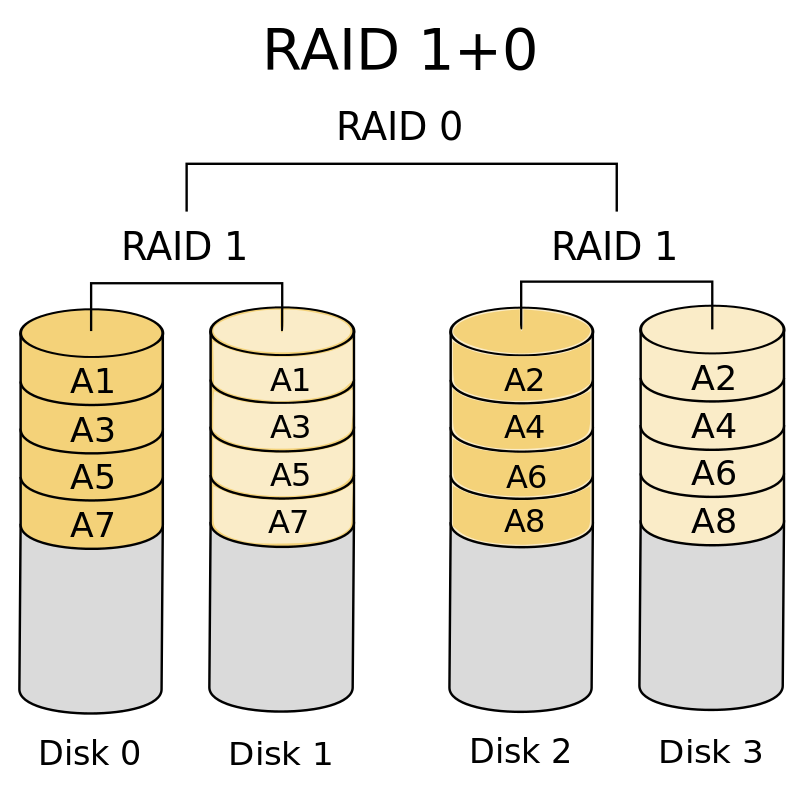
\includegraphics[scale=0.2]{raid10.png}
    \caption{RAID 1+0}
    \label{fig:my_label_8}
\end{figure}

RAID level is chosen mainly based on \textit{rebuild time} (time to rebuild the contents of a failed disk). Rebuild time is least for RAID 1, and most for RAID 5.\\


\subsection{RAID Implementation}
RAID can be implemented at the following layers
\begin{itemize}
    \item At the \textbf{kernel} or \textbf{system software} layer, using \textbf{volume management software}. Using minimum hardware features (and RAID 01 or 10 to avoid slow parity computations) a fully functioning RAID solution can be implemented.
    
    \item Using \textbf{Host Controller} hardware (also called the host-bus adaptor or HBA). Only the disks connected to the HBA can take part in RAID, hence this solution is not scalable. 
    
    \item In the \textbf{storage array hardware}, where the disks are split into RAID sets of various levels and even sometimes further sliced into volumes that are presented to the OS. The file system needs to be implemented on each volume only. Arrays can have multiple connections or be part of a Storage Area Network (SAN).
    
    \item In the \textbf{SAN interconnect layer} by disk virtualization devices. One controller between the hosts and the storage accepts commands from the servers and manages access to the storage. It could provide mirroring, by writing each block to two separate storage devices.

\end{itemize}

RAID implementations also offer external features like automatic \textbf{replication} of writes, saving \textbf{snapshots} of file systems (the last modified state of the file system) and \textbf{hot spares} (disks that are not used for data but can step in in case of disk failure, eg: rebuild a mirrored pair when one disk of that pair fails).

\subsection{Issues with RAID}
\begin{itemize}
    \item RAID is not capable of handling issues regarding incorrect/corrupt file pointers, incomplete writes (ie. corrupt data), and processes accidentally writing over the file system
    data structures.
    
    \item The \textbf{Solaris ZFS} file system makes use of \textbf{checksums} to verify data integrity. 
    
    \item The checksum value of a block is stored not inside that block, but rather with the pointer that points to that block. If a block is detected as having an incorrect checksum, then the mirrored copy of that block can be copied to that location with the correct data value.
    
    \item The overhead of checksum computation is not noticeable as the overall performance of ZFS is fast. The checksum computation provides more consistency and error detection+correction capabilities than normal RAID disks and file systems do. 
    
    \item RAID also lacks flexibility in file sizes (eg: 20 disks, in 4 groups of 5. Each group of 5 is in a RAID 5 set up, hence there are 4 volumes of disks each with their own file system. If one file is too large to fit on one volume then it can't be stored entirely on one volume. Similarly, small files will waste space). 
    
    \item In ZFS, disks (or partitions of disks) are available as contiguous storage that can be allocated using the model of \texttt{malloc()} and \texttt{free()}. These contiguous storage units are called \textbf{pools} of disks. 
    
    \item A pool can hold one or more ZFS file systems. 
    
    \item ZFS provides quotas to limit the size of a file system and reservations to assure that a file system can grow by a specified amount, but those variables can be changed by the file-system owner at any time.
\end{itemize}

\begin{figure}[!h]
    \centering
    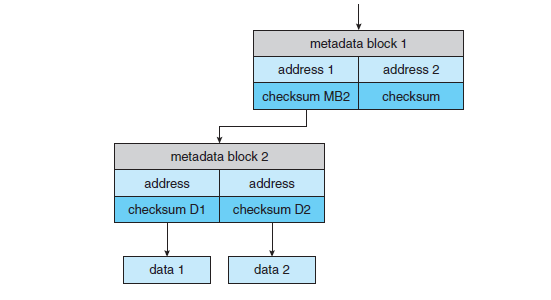
\includegraphics[scale=0.66]{os2.png}
    \caption{Storage in ZFS using checksums}
    \label{fig:my_label_14}
\end{figure}

\begin{figure}[!ht]
    \centering
    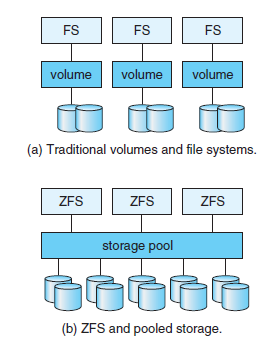
\includegraphics[scale=0.7]{os3.png}
    \label{fig:my_label_15}
\end{figure}

\section{File System: Concepts and Implementation}
\subsection{File}
\begin{itemize}
    \item A file is the smallest logical unit of data storage in a computer system. It is a named collection of related information that is stored on the secondary storage. 
    
    \item The attributes that define a file are:
    \begin{itemize}
        \item \textbf{Name}: A symbolic human-readable identifier for the file. 
        
        \item \textbf{Identifier}: the non human-readable name for the file, a unique index or identifier for it. 
        
        \item \textbf{Type}: For systems that support different file types.
        
        \item \textbf{Location}: Pointer to a device and the file's location on that device.
        
        \item \textbf{Size}: Current size (in bits/bytes/blocks) and maybe max allowed size stored as well.
        
        \item \textbf{Protection}: Read/write/execute permissions for different users on a file. 
        
        \item \textbf{Time, Date, user ID}: Timestamp and user at time of last modification of that file, used for protection, security or monitoring (billing info). 
    \end{itemize}
\end{itemize}

\subsubsection{File Operations}
\begin{itemize}
    \item File operations
    \begin{itemize}
        \item \textbf{Creating a file}: This involves allocation of disk space and then creating a directory entry.
        
        \item \textbf{Write to file}: A write system call needs the file name, and the information to be written to the file. For each file a \textit{write pointer} denotes the location of the next write within that file. The write pointer is updated after each write.
        
        \item \textbf{Read from file}: The read system call uses the file name and the memory address to which the read data is copied. The \textit{read pointer} is maintained for each file determines the location of the next read to take place. (NOTE: As most files are either being read or written at once and concurrent read/write is rare, only one \textit{file pointer} is maintained in most systems to save space and reduce complexity).
        
        \item \textbf{Repositioning or file seek}: No actual I/O involved, only manipulation of the file pointer.
        
        \item \textbf{Delete file}: Free the space occupied by the file, then remove the directory entry.
        
        \item \textbf{Truncating a file}: Keep all attributes of a file but only change the length. 
    \end{itemize}
    
    \item Operations like appending and copying are combinations of these 6 primitive file operations. 
    
    \item To repeatedly avoid searching in the directory for a given file name, the OS requires that file ops like read/write/seek take place only after executing an \texttt{open()} system call. 
    
    \item The OS maintains a cache of all the open files called the \textbf{open file table}. By directly indexing into the open file table, no searching is required anywhere.
    
    \item The \texttt{open()} call searches the directory structure and copies the file entry into the open file table. It returns a file pointer, so while the file is open the pointer is used for all operations. This reduces the need for searching the directory structure again. 
    
    \item There are 2 levels of open file tables: the per process table and the system-wide open file table. 
    
    \item Each entry in the per-process open file table points to an entry in the system wide open file table. Every time a new process opens an already opened file it points to the entry in the system-wide open file table.
    
    \item The system-wide file table maintains \textbf{file open count} for each open file that counts the number of processes that have opened that file. Each \texttt{open()} call increases the count and each \texttt{close()} call reduces it. When the file count goes to 0 the entry is removed from the system-wide open file table. 

\end{itemize}

\subsubsection{File Locks}
\begin{itemize}
    \item File locks are used to ensure mutual exclusion in file access. 
    
    \item \textbf{Shared locks} are like reader locks in that several processes can acquire them at once. 
    
    \item \textbf{Exclusive locks} are like writer locks in that only one process can acquire it at once. Exclusive locks prevent any other locks from being acquired on the file.
    
    \item Locks can also be either mandatory or advisory locks.
    
    \item \textbf{Mandatory locks} prevent other processes from acquiring an exclusive lock on a process once an exclusive lock has been acquired on that file. 
    
    \item \textbf{Advisory locks} allow other processes to manage locks themselves, but does not prevent them from accessing an already locked file. In this case, the process must be coded such that it acquires the lock manually. 
\end{itemize}

\subsection{File Structure}
\begin{itemize}
    \item Each file type has its own associated file structure that can be interpreted differently by the OS.
    
    \item The disadvantage of having too many file structures (for different file types) is the increased size and complexity of the resulting OS, and reduced flexibility with new file types and new applications.
\textit{    
}    \item All OSes support an executable file structure, but most OSes allow the application to define their own file structure, thus allowing flexibility. 
\end{itemize}

\subsubsection{Internal File Structure}
\begin{itemize}
    \item Logical divisions of files, called \textit{logical records} are packed into physical divisions on the disk called \textbf{blocks} (normally blocks correspond to sectors on the disk). 
    
    \item In UNIX, each logical record is one byte, and all files are streams of bytes. 
    
    \item Physical allocation of blocks can cause internal fragmentation if block size is too large (eg: a file of size 1949 bytes has to be allocated 4 blocks of 512 byte size with internal fragmentation of 99 bytes).
    
    \item Internal fragmentation increases as the block size increases.
\end{itemize}

\subsection{File Access Methods}
\subsubsection{Sequential Access}
\begin{itemize}
    \item A file here is treated as a \textit{tape}.
    
    \item One file pointer accesses logical records in sequential order. The \texttt{read\_next()} and \texttt{write\_next()} methods are used to access the current block and advance the pointer. The \texttt{reset()} method sets the file pointer to position 0 in the file
    
    \item On some systems the pointer can be made to move forward or backward $n$ blocks at a time where $n > 1$.
\end{itemize}

\subsubsection{Direct Access}
\begin{itemize}
    \item Logical records of the file are of fixed length, and they can be accessed in any order (no fixed sequence). 
    
    \item The \texttt{read(n)} and \texttt{write(n)} methods are used to access the file block numbered $n$. 
    
    \item The blocks are normally numbered according to their offsets from the beginning of the file, called the \textbf{relative block number}. 
    
    \item Sequential access can be simulated on a direct-access file by maintaining a current position \texttt{cp} variable. 
    
    \item The \texttt{read\_next()} operation on the direct access file is then equivalent to \texttt{read(cp)} followeed by \texttt{cp=cp+1}. 
    
    \item The \texttt{write\_next()} operation on the direct access file is then equivalent to \texttt{write(cp)} followeed by \texttt{cp=cp+1}. 
\end{itemize}

\subsubsection{Indexed Access}
\begin{itemize}
    \item The index is a data structure that contains a key and a pointer to the file record corresponding to that key. 
    
    \item First the index is searched by key, and then the appropriate file record can be accessed from its pointer.
    
    \item In order to prevent the index table from becoming too large, the index table can be nested (ie. index table pointing to sub index table entries that in turn point to file blocks). 
\end{itemize}

\section{Directory Structure}
\begin{itemize}
    \item A \textbf{volume} is a unit of disk space that holds a file system. 
    
    \item A volume can correspond to a subset of a device, an entire device or multiple devices in RAID. A volume can also hold multiple Operating Systems. 
    
    \item Each volume holds information about the files in it in a data structure called the \textbf{device directory} or the \textbf{volume table of contents}. 
\end{itemize}

\subsection{Directory Organization}
\begin{itemize}
    \item File systems are complex and of many different types. eg: the file system types in Solaris are as follows:
    
    \begin{itemize}
        \item \textbf{ufs, zsf}: General Purpose FS.
        
        \item \textbf{objfs}: A file system interface into the kernel, allowing developers access to the kernel symbol table.
        
        \item \textbf{tmpfs}: FS held in main memory, for caching purposes. 
        
        \item \textbf{ctfs}: Virtual FS that maintains "contract" information to manage which processes start when the system boots and must continue to run during operation
        
        \item \textbf{lofs}: Loopback file system, that allows a file to be mounted as if it were a physical device. 
        
        \item \textbf{procfs}: A virtual FS that represents all process information as a FS.
    \end{itemize}
\end{itemize}

\subsection{Directory Operations}
\begin{itemize}
    \item \textit{File operations}: Create, delete and rename files within a directory.
    
    \item \textit{Search directory for file}: Search by name, or search all files whose names match some pattern. 
    
    \item \textit{Traverse from root to leaf}: In order to make backup copies of a file system, or to free space occupied by non-used files.
    
    \item \textit{List contents of a directory}
\end{itemize}

\subsection{Logical Structure of Directories}
\subsubsection{Single Level Directory}
\begin{itemize}
    \item All files are stored in one single directory. All users share this directory. 
    
    \item This does not allow multiple users to store files with the same name on the machine. 
\end{itemize}

\subsubsection{Two Level Directory}
\begin{itemize}
    \item Each user has an associated \textbf{user file directory (UFD)}, which is a single level directory.
    
    \item The \textbf{master file directory} is indexed by the user ID and points to the UFD of that user. 
    
    \item All file system operations are confined only to the UFD of the currently active user. 
    
    \item If users are independent, this is an advantage. If users wish to collaborate on some project then this is a drawback, as systems do not allow one user to manipulate another user's UFD. 
    
    \item File names are specified as a combination of the UFD name and the file name (eg: \texttt{user1/t1.txt}). 
    
    \item The volume name can also be added to the file name (eg: on Windows \texttt{C:\textbackslash user1\textbackslash t1.txt}). 
    
    \item The problem with accessibility of other user's files is also prominent in system files. A copy of all the system files has to be kept in each UFD for the system programs to work. This is a waste of space.
    
    \item This is resolved by keeping a separate UFD for system files only, and using it as a last resort if the file name is not found in the current UFD. 
\end{itemize}

\subsubsection{Tree Structure Directory}
\begin{itemize}
    \item This is the multilevel extension of the two level scheme. 
    
    \item Each entry in a directory is either a file or a sub-directory (indicated by a bit in the directory table, 0 for file, 1 for sub-directory).
    
    \item Each process has a \textit{current directory} where its files of interest are stored. 
    
    \item The \texttt{change\_directory()} system call changes the current directory. 
    
    \item The initial directory for each user is stored in some fixed location (\texttt{/etc/passwd} for Linux systems). Once the shell is launched from this location, processes can be spawned. 
    
    \item File paths can be \textit{relative} (wrt. to the current directory) or \textit{absolute} (wrt. the root of the FS). 
    
    \item On some systems, non-empty directories cannot be deleted. On other systems, the file system offers the option to clean all files and subdirectories recursively on its own to the user (eg: in the Linux \texttt{rm} command). 
    
    \item All users can access each others files using absolute or relative paths (by changing the current directory). 
\end{itemize}
\begin{figure}
    \centering
    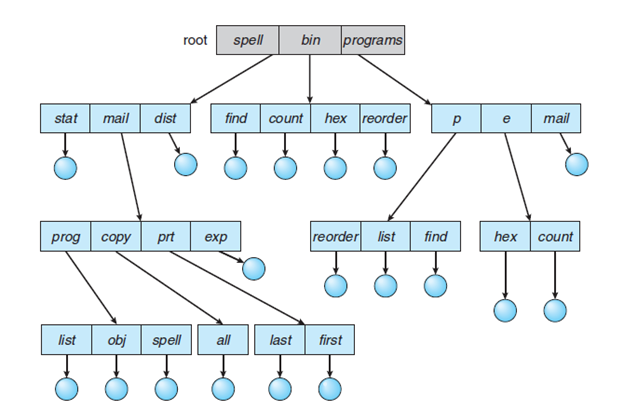
\includegraphics[scale=0.8]{os4.png}
    \caption{Tree Directory Structure}
    \label{fig:my_label_13}
\end{figure}

\subsubsection{Acyclic Structure Directory}
\begin{itemize}
    \item This structure allows a single file or directory to exist in multiple directories. 
    
    \item This is implemented in UNIX as a \textbf{link}. A link is a special directory entry that contains the true path of the file it points to. It is essentially an indirect pointer. 
    
    \item In order to maintain the acyclic property of the FS, links are ignored while traversing the file system. 
    
    \item Shared files can also be implemented by having duplicate directory entries in all the directories that hold it. But this has the issue of consistency when one user modifies the file. 
    
    \item  Multiple file paths now can refer to the same file name. This causes issues when the file system is to be traversed. 
    
    \item When a file is deleted, the management of links becomes an issue, as it may lead to dangling pointers. 
    
    \item With symbolic links the issue of deletion is simple. If a link is deleted, then the file is not affected but the link is cleared. If the original file itself is deleted then the link becomes dangling, 
    
    \item In Windows and UNIX, the user is left to deal with such dangling links. 
    
    \item Another approach to file deletion is to only delete links, and delete the actual file only when there are no references to it anymore (this means that a reference count or a list of references to each file has to be maintained). 
    
\end{itemize}

\begin{figure}
    \centering
    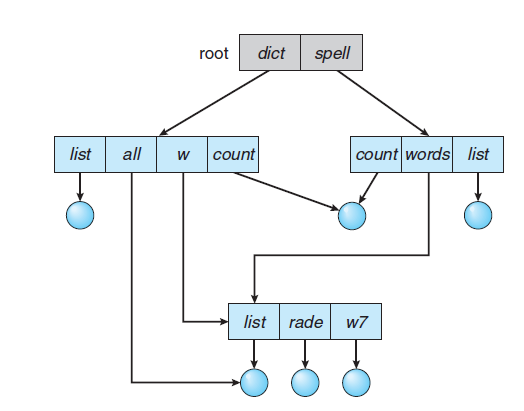
\includegraphics[scale=0.8]{os5.png}
    \caption{Acyclic Structure}
    \label{fig:my_label_16}
\end{figure}

\subsubsection{General Graph Structure}
\begin{itemize}
    \item If cycles are formed in the structure, then algorithms for traversal can get stuck in an infinite loop in accessing these cycles.
    
    \item Some sections of the structure may be accessed multiple times unnecessarily because of the presence of cycle.
    
    \item One solution is to arbitrarily limit the number of directories that can be accessed in a single traversal. 
    
    \item In an acyclic graph, if the reference count of a file/directory is 0 then it can be safely deleted. But the existence of cycles means that reference count may be 0 even when no other references exist (this occurs due to the possibility of sel referencing).
    
    \item \textbf{Garbage collection} mechanisms traverse the tree structure, and mark all the accessible nodes. The second traversal gathers all the unmarked nodes into a list of freeable disk space and then deletes those nodes. 
    
    \item This is time consuming on disk-based file systems. 
    
    \item Cycle detection algos are expensive to run on disk especially, hence acyclic structures are preferred. Links are simply ignored while traversing. 
\end{itemize}

\section{File System Mounting}
\begin{itemize}
    \item Mounting is the process of associating a file system on an external device, with the Operating System so that the users can access it.
    
    \item The OS needs the device name, the mount point (the directory in the OS where the device will be mounted, normally an empty one), and the file system type of the file system that is to be mounted. 
    
    \item The file system is an optional argument, some OSes can automatically detect which file system is being used on the device. 
    
    \item In Windows and UNIX based OSes, the OS discovers all the connected devices and mounts them at boot time. 
    
    \item In systems where the \texttt{mount} command is explicitly used, the pre-defined mount points at boot time are located in a system config file (\texttt{/etc/fstab} on Linux systems). 
\end{itemize}

\section{Shared Files}
\subsection{Multi-User Control}
\begin{itemize}
    \item Security is maintained through a file \textbf{owner} and a \textbf{user group}.
    
    \item The owner can modify permissions and attributes of the file. The group is the subset of users that are allowed to modify the file. 
    
    \item User manipulation of files involves first checking if the user is the owner, and then if the user belongs to the group that can modify the file. 
\end{itemize}

\subsection{Remote File Systems}
\begin{itemize}
    \item The earliest implementations were manual file transfer using the \texttt{ftp} protocol. 
    
    \item The next advancement in this area involved \textbf{Distributed File Systems} (DFS) where remote directories were visible from local machines. 
    
    \item The current method for remote file access is the world wide web, that uses HTTP for file transfer.
    
    \item \textit{Anonymous access} is a method that allows a user to access a remote file system without having an account on the remote system. This is used in HTTP, while ftp is capable of both anonymous and authenticated access.
    
    \item DFS involves tighter integration between the two systems that exchange files. 
\end{itemize}

\subsubsection{Client-Server Model}
\begin{itemize}
    \item The client seeks the files that are stored on the server machine. 
    
    \item Clients are identified by their network or IP Address. As the IP Address can be \textit{spoofed}, thus allowing an unauthorized client access to files on the server. 
    
    \item Security methods like public key encryption are possible but hard to implement as they need the negotiation of a secret key between both machines. 
    
    \item On the UNIX Network File System (NFS), the authentication is checked based on the user ID on server and client (for one user, they should be same on both machines). 
    
    \item NFS allows many-to-many client server relationships. A machine can act as an NFS client or an NFS server at the same time. 
    
    \item Once the remote NFS is mounted, the DFS protocol ensures that requests for opening, closing and other file ops are sent along with the correct user ID. 
\end{itemize}

\subsubsection{Distributed Information Services}
\begin{itemize}
    \item This service allows hosts to identify each other with their network addresses. (eg: DNS on internet)
    
    \item It can also be used to store authentication information for users using a shared file system. Sun Microsystems introduced this service as \textbf{yellow pages} or \textbf{Network Information System} (NIS).
    
    \item NIS uses unencrypted transmission of sensitive data including passwords. NIS+ makes this secure using encryption but increases overheads and complexity of the resulting service. 
    
    \item In Microsoft's \textbf{Common Internet File System} (CIFS) the network info is used along with user info (ID and password) to create a network login that is used by server to authenticate permissions for files. 
    
    \item CIFS uses \textbf{active directory} to provide a single name space for all users.
    
    \item The industry standard currently is \textbf{Lightweight Directory Access Protocol} (LDAP). Theoretically, a single distributed LDAP directory is used for all user authentication info storage.
    
    \item The end result is a single sign-in for users to be able to access all the systems in the network, that increases convenience while reducing the efforts of system administration. 
\end{itemize}

\subsubsection{Failure Modes}
\begin{itemize}
    \item Local file systems can suffer from hardware component failure (disk failure, host adaptor failure, disk controller failure, cable failure), data corruption on disk (file system corruption, metadata corruption) or system failure that leads to directory deletion by mistake.
    
    \item Remote File Systems also have network related failures (due to bad hardware or bad configuration) in addition to these.
    
    \item The remote file system protocols allow for DFS commands to be terminated or simply delayed until the resource is online once more. The latter is the more common option.
    
    \item The recovery of lost servers in a remote file system is done by maintaining \textit{state information} on client and server. If both maintain knowledge of their open files and all operations, then recovery can be easily done. 
    
    \item NFS simplifies the design by assuming that all file operation requests are legitimate (ie. the volumes were correctly mounted on the client, and the respective files were open). This means that the NFS can now be made \textbf{stateless}.
    
    \item The disadvantage of a stateless design is the reduced security, as read/write requests can be forged by unauthorized users while the NFS is in failure mode. 
    
    \item In NFS v4, the NFS is made \textbf{stateful} to solve the above issue.
\end{itemize}

\subsubsection{Consistency Semantics}
\begin{itemize}
    \item Evaluate file system consistency when simultaneous access of one file happens by multiple users. 
    
    \item \textbf{UNIX consistency semantics}:
    \begin{itemize}
        \item Writes to an open file are immediately visible to all users
        
        \item One file sharing mode ensures that the file pointer manipulated by one user is visible to all users. Hence the file acts as a single exclusive resource for which multiple users must fight for contention.
    \end{itemize}
    
    \item \textbf{Andrew's File System semantics}:
    \begin{itemize}
        \item Writes to an open file by a user are not visible immediately to other users that have the same file open.
        
        \item Changes made to a file are visible only in sessions that start after the current session. 
        
        \item One file is temporarily associated with multiple images at once, thus allowing each user to access the file with no delay. 
    \end{itemize}
    
    \item \textbf{Read-only semantics} (or immutable shared file semantics)
\end{itemize}

\subsection{File Protection}
\begin{itemize}
    \item Protection is implemented as an \textbf{Access Control List} (ACL), which is a list of operations that each user is allowed to perform on that file/directory.
    
    \item If the number of users is dynamic, then the directory entry has to be of variable size, and it can become a tedious task to configure permissions for all files for all users. 
    
    \item The solution is to have 3 groups of permissions for each file: the \textbf{owner} creator of the file), the \textbf{group}(users collaborating on the file, need similar access) and the \textbf{universe} (set of all users on the system).
    
    \item Most OSes combine both these functionalities, with more generic control from the groups and more fine-grained control coming from the ACL. 
    
    \item On UNIX and Linux systems the groups and their privileges are stored in groups of 3 bits (for read, write and execute permissions).
    
    \item Another approach to file protection is password protection. If passwords are assigned randomly and changed frequently then this is viable.
    
    \item Having different passwords for each file leads to a prohibitively large number of passwords for the user to remember, and having the same password for all files leads to lower security. 
\end{itemize}

\section{File System Structure}
\begin{itemize}
    \item The file system is organized as a layered system. 
\end{itemize}

\begin{figure}[!h]
    \centering
    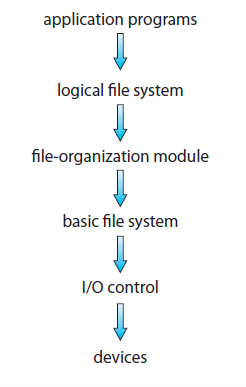
\includegraphics[scale=0.7]{os6.png}
    \caption{Layered Architecture of File System}
    \label{fig:my_label_17}
\end{figure}
\begin{itemize}
    \item The \textbf{I/O control layer} consists of Interrupt handlers and the device drivers for each storage device. 
    
    \item The device driver takes high level commands as input and outputs low level, hardware-specific commands for the disk controller to understand. 
    
    \item The \textbf{Basic File System} issues commands to the appropriate device driver to read and write specific blocks. 
    
    \item The BFS layer also manages buffer space for I/O (all blocks are written to the buffer before it is written to the disk, if the buffer is full then space must be freed up) and cache memory for I/O operations (for frequently used file system metadata, to increase performance).
    
    \item The \textbf{file organization module} translates logical block addresses within a file (0 to $N$) to actual physical block addresses on disk. 
    
    \item The File Organization Module also includes the free space manager that tracks unallocated blocks and offers them when requested.
    
    \item The \textbf{logical file system} manages file system metadata. It manages the directory structure, and the file structure using \textbf{file control blocks} (also called \textbf{inodes} on UNIX file systems). 
    
    \item FCBs hold file info like ownership, permissions, and location of the file. It is also responsible for protection. 
\end{itemize}

\subsection{Implementation}

\subsubsection{Disk Structures}
\begin{itemize}
    \item \textbf{Boot Control Block}: Contains the info needed to boot an OS from that volume. It is the first block in the volume, and it is called the \textbf{partition boot sector} in NTFS or \textbf{boot block} in UFS.
    
    \item \textbf{Volume Control Block}: contains partition/volume info like block size, number of blocks in the volume, number of free blocks and a list of free block pointers. UFS refers to this as a \textbf{superblock}, while NTFS stores this info in the \textbf{master file table}. 
    
    \item \textbf{Directory Structure} to organize files. In UFS this includes the file names and their associated inode numbers. In NTFS this is stored in the master file table.
    
    \item \textbf{File Control Blocks} for each file. Each FCB has a unique number that associates it with a directory entry. In NTFS this is also stored in the master file table that uses a relations DB structure.
\end{itemize}

\subsubsection{In-Memory Structures}
\begin{itemize}
    \item \textbf{Mount table} stores info about mounted volumes. 
    
    \item \textbf{Directory Cache} stores directory entries of recently accessed directories. 
    
    \item \textbf{System wide open file table} and \textbf{Per-process open file tables}. The system wide table contains a copy of the FCB of the open file,and the per process table contains pointers to the entries in the system-wide table. 
    
    \item \textbf{Buffers} to hold data while being written to/read from disk. 
\end{itemize}

\begin{figure}[!h]
    \centering
    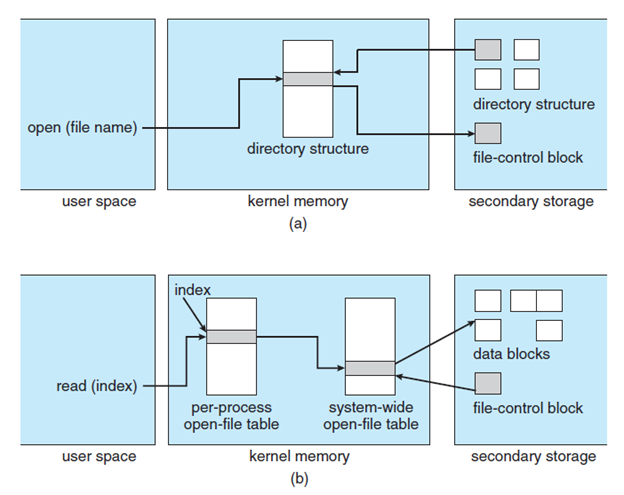
\includegraphics[scale=0.7]{os7.png}
    \caption{a) File open b) File reading}
    \label{fig:my_label_18}
\end{figure}

\subsubsection{File Creation}
\begin{itemize}
    
    \item The program calls the logical file system that knows the directory structure and the FCB format.
    
    \item A new FCB is created (or allocated from a pool of empty FCBs).
    
    \item The appropriate directory is read into memory, updated with the file name and the new FCB, and then written back to disk.
\end{itemize}

\subsubsection{File Opening}
\begin{itemize}
    \item The \texttt{open(filename)} system call is used to open files. It first checks the system-wide open file table for a match. 
    
    \item If the corresponding entry exists in the system-wide open file table, then a pointer to that entry is added in the per-process open file table.
    
    \item If it does not exist, then the directory structure is checked for the file. The appropriate FCB is loaded onto the system-wide open file table. 
    
    \item Once the system-wide table conains the FCB, pointer to that entry is added in the per-process open file table (along with info like a pointer to the current location in file for read/write, and the current process' access mode). 
\end{itemize}

\subsubsection{Closing File}
\begin{itemize}
    \item The entry in the per process file table is removed
    
    \item The reference count in the system wide file table is reduced by 1.
\end{itemize}

\subsection{Partitioning and Mounting}
\begin{itemize}
    \item A \textbf{raw partition} is one that does not have a file system on it (used for swap space, or databases holding RAID metadata like blocks that are mirrored and need to be updated etc.)
    
    \item A \textbf{cooked partition} contains a complete and correct file system. 
    
    \item The boot info is stored in a separate boot partition. The bootloader is stored in this partition. It knows the location of the kernel so that it can be loaded and start executing. 
    
    \item The boot partition is responsible for mounting the \textbf{root partition}. The root partition contains the kernel and other system files.
    
    \item The system verifies the integrity of the root partition by asking the device driver to check the device directory and its format. In case of a wrong format, the consistency of the root partition is checked and corrected (without user intervention). 
\end{itemize}

\subsection{Virtual File System}
\begin{itemize}
    \item This is a translation layer between the OS-specific system calls for file handling, and the appropriate commands for the specific file system that is mounted there.
    
    \item It allows multiple file systems to be mounted on one computer, and allows the user to seamlessly switch between them. 
    
    \item The functions of the VFS layer are:
    \begin{enumerate}
        \item Separate generic file system operations from their specific implementations
        
        \item Provide an unique representation of a file throughout a network, using the concept of \textbf{vnodes}. Vnodes are identified by the vnode number that is unique throughout the network (not just unique to one file system, like inodes are). 
    \end{enumerate}
    
    \item The object types recognized by the VFS are:
    \begin{enumerate}
        \item \textbf{inode} object that represents a single file
        
        \item \textbf{dentry} object represents a single directory entry.
        
        \item \textbf{file} object represents an open file
        
        \item \textbf{superblock} object represents an entire file system. 
    \end{enumerate}
    
    \item The VFS defines specific functions that are unique for each of these types. 
    
    \item These structures contain pointers to a function table that itself contains pointers to the functions for the types. 
\end{itemize}

\subsection{Directory Implementation}

\subsubsection{Linear List}
\begin{itemize}
    \item This is a list of file names with pointers to the blocks on disk.
    
    \item Creating a file involves searching the directory structure to see that it does not already exist, then creating a new list entry at the end.
    
    \item Deleting a file involves searching the directory structure again, and releasing the space allocated to that file. 
    
    \item The disadvantage of linear list is that searching takes $O(n)$ time. If the list is kept in sorted order this can be made to $O(log_2n)$ time but creation and deletion of files in the sorted list is more complex. 
    
    \item More complex data structure like balanced trees (AVL/Red-Black/B Trees) can be used in this case. 
\end{itemize}

\subsubsection{Hash table}
\begin{itemize}
    \item The hash table is used for quick search in the linear list of files.
    
    \item The hash function takes in the file name and returns a pointer (ie. an index) to the file entry in the list.
    
    \item Searching in this case becomes $O(1)$ operation. 
    
    \item Collisions can occur due to the hash table not being of sufficient size. Collisions can be handled either by linear probing, or chaining (wherein each entry of the list is itself a linked list of entries having the same hash value). 
    
    \item Increasing the hash table size is complicated as the hash function depends on the size, hence the entire list has to be reorganized by the new hash function. 
\end{itemize}

\subsection{Disk Space Allocation}

\subsubsection{Contiguous Allocation}
\begin{itemize}

    \item Contiguous allocation is defined by the address of the first block and the block size. 
    
    \item Given the start block and the length of the file, the blocks are allocated continuously after it. 
    
    \item Contiguous allocation supports both sequential and direct access methods. For sequential access, the file system remembers the current location of the file and all reads/writes take place from that position. For direct access, as the file system knows the start address of the file it can easily access any block by doing pointer arithmetic (addr of block i = $b+i$).
    
    \item Free space management is done using either first fit, best fit or worst fit. All these methods suffer from external fragmentation. 
    
    \item Compaction is done to solve external fragmentation. The file system is copied to another disk. Then the files on the temp disk are allocated from this large free space such that there are no holes. 
    
    \item Compaction leads to a performance penalty, hence it is done during the \textit{down time} or the \textit{off time} of the system. 
    
    \item Another drawback of contiguous allocation is knowing in advance the length of the file and allowing space for it to grow. 
    
    \item Methods to solve this:
    \begin{enumerate}
        \item Repeated runs of the file with different allocations, wasteful in terms of memory and CPU usage. 
        
        \item Copy contents to a larger hole and free the old space. This leads to wasted space and internal fragmentation. 
    \end{enumerate}
    
    \item Some FS allow the user to add another fragment to the end of the contiguous allocated block, called an \textbf{extent}. The extent allocation may lead to internal fragmentation if the extent size set by the user is too large.
\end{itemize}

\begin{figure}
    \centering
    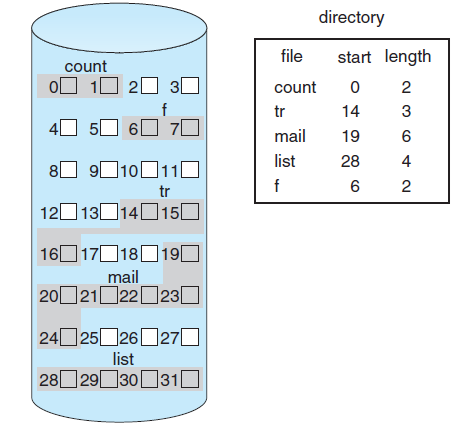
\includegraphics[scale=0.6]{os8.png}
    \caption{Contiguous Allocation}
    \label{fig:my_label_19}
\end{figure}

\subsubsection{Linked Allocation}
\begin{itemize}
    \item Blocks on disk are allocated in a non-contiguous manner like a linked list. Every block has a pointer to the next block in the file.
    
    \item Out of each block some space will have to be reserved for this pointer. (eg: block size 512 bytes, and pointer size of 4 bytes implies that 508 bytes will be used for actual data).
    
    \item File size does not have to be mentioned in this scheme. As long as empty blocks are available they can be added to the end of the file and the file can grow. 
    
    \item The disadvantage is the space taken up by the pointers, and the difficulty in implementing direct access for files in this scheme (in order to directly access block $i$ of the file the disk head must start from the beginning of file and traverse $i-1$ pointers to reach there). 
    
    \item The solution is to allocate at the \textbf{cluster} level instead of the block level. A cluster is a contiguous collection of blocks. 
    
    \item The advantages of cluster allocation are less number of disk head seeks needed leading to higher disk throughput, and reduced overhead for block allocation and free list management.
    
    \item The disadvantage of cluster allocation is increased internal fragmentation.
    
    \item Another disadvantage of linked allocation is reliability and fault tolerance. If one of the pointers is corrupted due to a bug in the device driver or the OS then the wrong block (maybe empty or belonging to another file) will be picked up.
    
    \item The solution (with the penalty of increased overheads) are to use a doubly linked list, and to have file name and relative block number info stored on each file block.
\end{itemize}

\subsubsection{File Allocation Table}
\begin{itemize}
    \item This is a variation of the Linked allocation scheme. The beginning of every volume is allocated for the FAT. 
    
    \item The FAT is indexed by the block number, and contains one entry for each block in the disk. 
    
    \item The directory entry for a file contains the index of the first block in the FAT. The entries of the FAT contain the index of the next block in the file for each entry. 
    
    \item The last block of the file is a special EOF block that has 0 value. 
    
    \item The FAT causes disk seek overheads (as the head has to move to the beginning of the disk to read the FAT for each block access). The FAT speeds up direct access as it stores information regarding each block's location. 
\end{itemize}

\begin{figure}[!h]
    \centering
    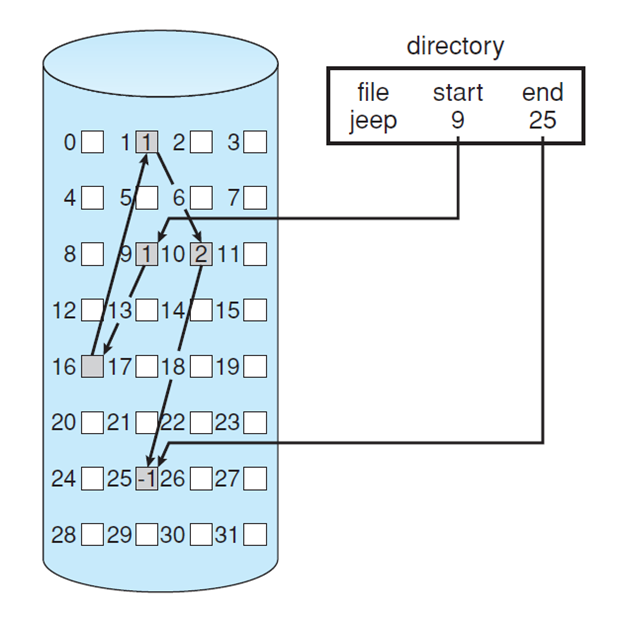
\includegraphics[scale=0.5]{os9.png}
    \caption{Linked Allocation}
    \label{fig:my_label_20}
\end{figure}

\begin{figure}[!h]
    \centering
    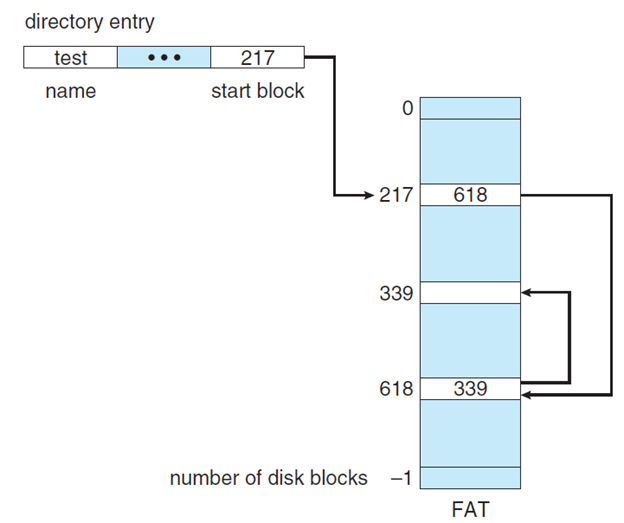
\includegraphics[scale=0.5]{os10.png}
    \caption{File Allocation Table}
    \label{fig:my_label_21}
\end{figure}

\subsubsection{Indexed Allocation}
\begin{itemize}
    \item All the files now have a separate \textbf{index block}. The index block contains a table of pointers to all the blocks in the file.
    
    \item The index table is stored in order. The ith table entry is the poiinter to the ith file block. 
    
    \item Initially all pointers are set to \texttt{NULL}. The ith block is modified as it is allocated. 
    
    \item Indexed allocation supports direct access without external fragmentation. Indexed allocation, however, suffers from pointer overheads larger than linked allocation. 
    
    \item Index block size limits the size of the file. Solutions to this are:
    \begin{enumerate}
        \item \textit{Linked} index blocks together for large files.
        
        \item \textit{Multilevel} index blocks, with primary index block pointing to secondary index blocks and so on. 
        
        \item \textit{Combined scheme}: Used in UNIX file systems. The first 15 pointers of the index block are stored in the Inode. The first 12 are \textit{direct pointers} to file blocks. The next 2 are \textit{single indirect} pointers that point to index blocks that point to data. The last one is a \textit{double indirect} pointer that adds another level of indirection to the first. 
    \end{enumerate}
\end{itemize}

\begin{figure}[!h]
    \centering
    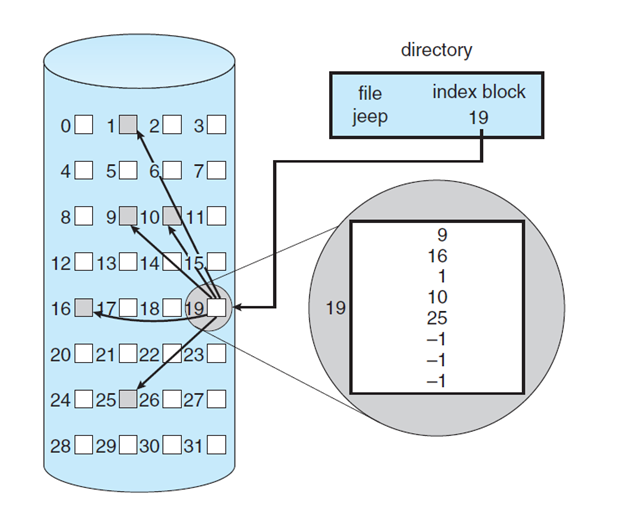
\includegraphics[scale=0.5]{os11.png}
    \caption{Indexed Allocation}
    \label{fig:my_label_22}
\end{figure}

\begin{figure}[!h]
    \centering
    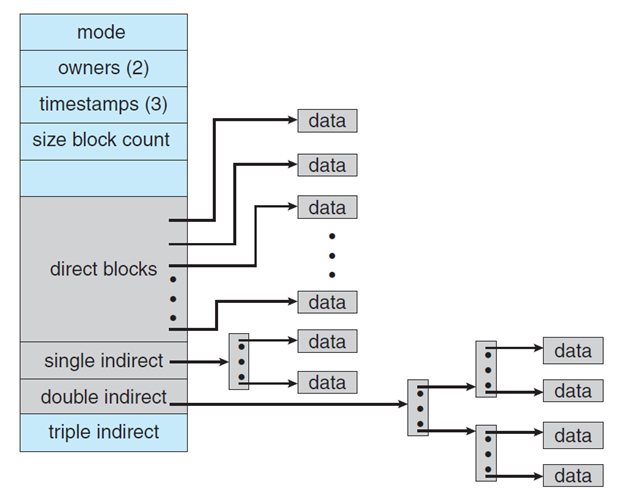
\includegraphics[scale=0.5]{os12.png}
    \caption{UNIX Inode structure with pointers}
    \label{fig:my_label_23}
\end{figure}


\end{document}

